
% INTRODUCCION
	\section{Introducción}
		Puedo hablar lo que puse al final de mi presentación de la tesis.

% METODOS
	\section{Métodos}

	\subsection{Exposición del detector}

	Si consideramos la variación de la exposición del observatorio durante $t_{i}$ y $t_f$, debido al crecimiento del SD o por periodos de mal funcionamiento de arreglo, modula el número de 	eventos en función del tiempo. 
	
	Para hacer el peso sigo los siguientes pasos
	\begin{enumerate}
		\item Selecciono un rango de tiempo entre $t_i$ y $t_f$.
		\item Para un periodo de tiempo $T$ en días SIDEREOS (365.25 dias normales a 366.2559 dias sidereos) , lo trasformo a  años {\bf SIDEREOS}  o vueltas, para ir barriendo las 24 hrs SIDEREAS de la ascensión recta con el periodo que estoy estudiando.
		\item Voy sumando la cantidad de tanques por cada hora que voy recorriendo. 
		\begin{equation}
			N_{tanques}(t) = \sum_j n_{tanques}(t + jT)
		\end{equation}
		\item Después de obtener las suma de los tanques , hago la ``integral'', es decir, vuelvo a sumar pero sobre las 24 horas (sidereas),  
		\begin{equation}
			I_{tanques} = \frac{1}{T} \int_{0}^{T} dt \, N_{tanques}(t) \rightarrow I_{tanques} = \sum^{288}_{t_{siderea=1}}\frac{ N_{tanques}(t_{siderea})\times5\, \text{min}}{288 \times 5\, \text{min}}
		\end{equation}
	
		\item Luego se puede calcular $\Delta N_{tanques}$ para cada hora sidérea, mediante la siguiente expresión
	
		\begin{equation}
			\Delta N_{tanques}(t) = \frac{N_{tanques}(t)}{I_{tanques}}
		\end{equation}
	
		\item Posteriormente, uno puede calcularse el peso  $w_i$ correspondiente a un evento que ocurrió a un horario (sidereo) $\tau$, mediante la siguiente expresión
		\begin{equation}
			w_i = \frac{1}{\Delta N_{tanques}(\tau)} 
		\end{equation}
		En la práctica, $\tau$ corresponde a un valor entre 0 y 287, por lo que cada intervalo de 5 min  en hora siderea tiene un peso distinto .
	
	\end{enumerate}
	
	\emph{Intenté hacerlo sin tener en cuenta y lo que sale es una convolución de frecuencia y no tengo nada físico. 20/02/2020}

	Ahora lo estoy haciendo en un span de 5 min. (24/02/2020)

	\begin{figure}[H]
		\centering
		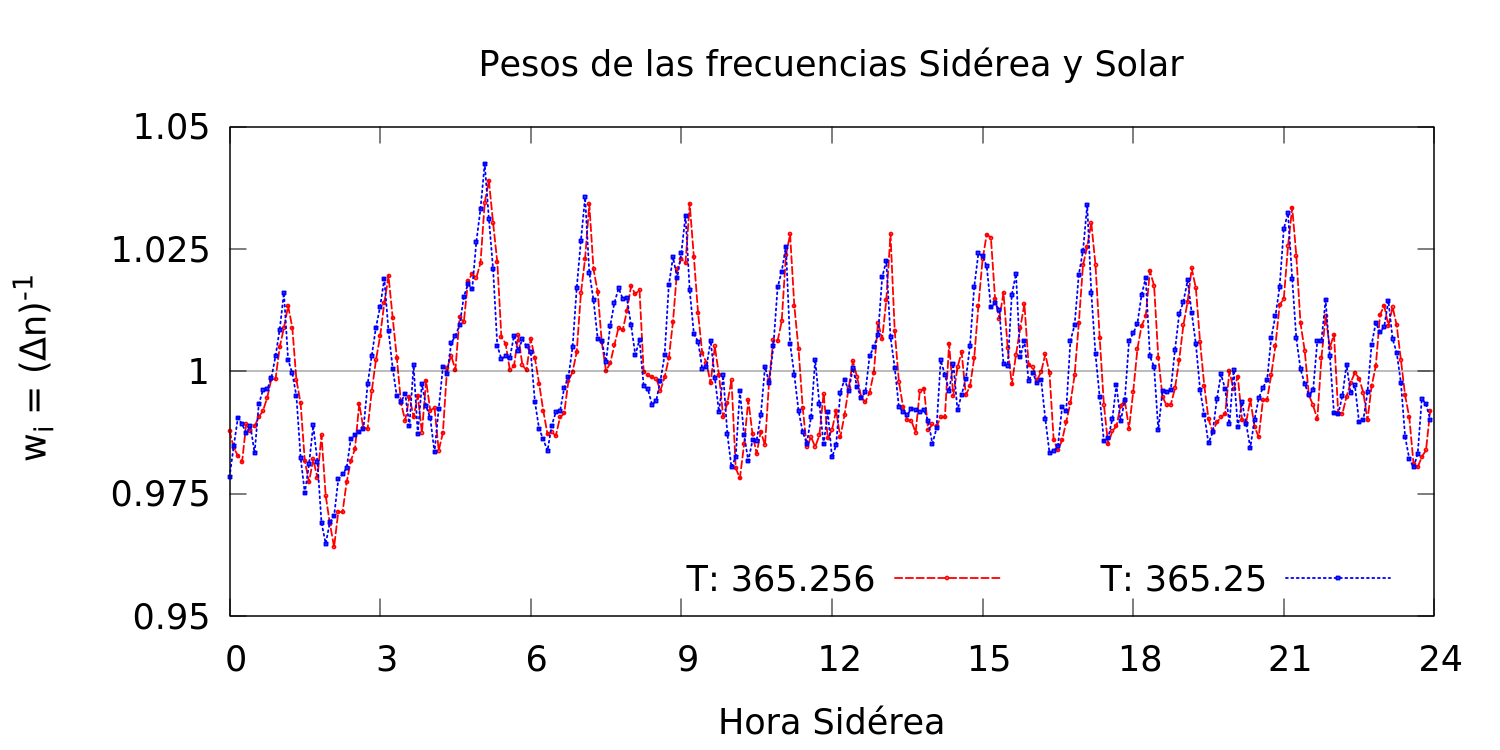
\includegraphics[width=0.95\textwidth]{../Anisotropia/pesos_solar_siderea.png}
		\caption{Pesos para dos frecuencias en particular, la frecuencia sidera y solar, de periodo $365.256$ y $365.25$ respectivamente}
		\label{fig:pesos_ejem}
	\end{figure}

	En la Fig.\ref{fig:pesos_ejem} se observa que el peso oscila alrededor de 1.

	\subsection{Análisis en ascensión recta}
	
	\begin{itemize}
		\item Ya cuando tengo los pesos $w_i$, el valor de N es $N=\sum_i w_i$
	
		\item La eficiencia del SD varía con la energía del CR. Para el disparo estandar, los eventos con energía mayor a $3\,$EeV y $\theta_{max}<60^o$ o 	por encima de $4\,$EeV y $\theta_{max}<80^o$, son detectados con una eficiencia del 100\%. Para todos los disparos, la eficiencia completa de 	alcanza por encima de 1\,EeV.
	
		\item Por lo tanto sin trabajamos con eventos donde la eficiencia es completa y sólo puede afectar el cambio de la exposición del observatorio, y  	no es necesario tener en cuenta en el peso la eficiencia.
	
		\item Para calcular el percentil 99, se usa que $P(>r) = \exp(\nicefrac{-N\,r^2}{4})$, por lo tanto para el valor de $r_{99\%}$ del percentil 99 $r	_{99\%}=\sqrt{-4\,\ln(0.01)/N}= \sqrt{4\,\ln(100)/N}$. Cabe resaltar que el P99 depende solamente de la cantidad de eventos que se se está estudiando. La interpretación 	de este valor es cual es la probabilidad de tener una amplitud mayor como una fluctuación de una distribución isotrópica.
	
		\item Para el análisis de Rayleigh, que describe el paper \cite{linsley1975fluctuation} se toma que  
		\begin{equation}
			a_\alpha = \frac{2}{N} \sum^{all}_i w_i \cos(\alpha_i)  \qquad	\qquad	b_\alpha = \frac{2}{N} \sum^{all}_i w_i \sin(\alpha_i)
		\end{equation}
	
		Donde $\alpha_i$ es el valor de la ascensión recta del evento. Para la amplitud  $r_\alpha$ y la fase $\phi_\alpha$ de cada evento
		\begin{equation}
			r_\alpha = \sqrt{a_\alpha^2 +  b_\alpha^2} \qquad \tan{\phi_\alpha} = \frac{a_\alpha}{b_\alpha}
		\end{equation}
	\end{itemize}


% ARCHIVOS DE DATOS Y SUS DIFERENCIAS
	\section{Características de los datos}

% RESULTADOS PARA ANISOTROPÍAS EN RA PARA LOS ICRC
	\section{Anisotropías en ascensión recta en los archivos del ICRC 2017 y ICRC 2019}

% ---> 8 EeV 
		\subsection{Eventos por encima de 8 EeV }

% ------> CARACTERISTICAS
			%\subsubsection{Características de los datos analizados}

% ------> ICRC 2017
			\subsubsection{Resultados para los datos del ICRC 2017}

			Para este apartado analicé el archivo de datos de la tesis de doctorado de Oscar Taborda, solamente los eventos 6T5. El rango de tiempo en el cual hice  el análisis es entre 1072969615 y 1472688000 (	2004-01-01 15:06:55 y 2016-11-01 0:00:00 )

			Sabemos que para energía mayores de 8 EeV, aparece el dipolo en sidérea.

			En las Fig.\,\ref{fig:8EeV_sin_peso_ICRC2017_raw} y \ref{fig:8EeV_sin_peso_ICRC2017_cor} se muestra la amplitud del primer armónico sin considerar el peso de los hexágonos. Está figura es compatible con la Fig. 5.7.b, página 90 de la tesis de Taborda.

				\begin{figure}[H]
				
					\begin{subfigure}[b]{\textwidth}
					\centering
						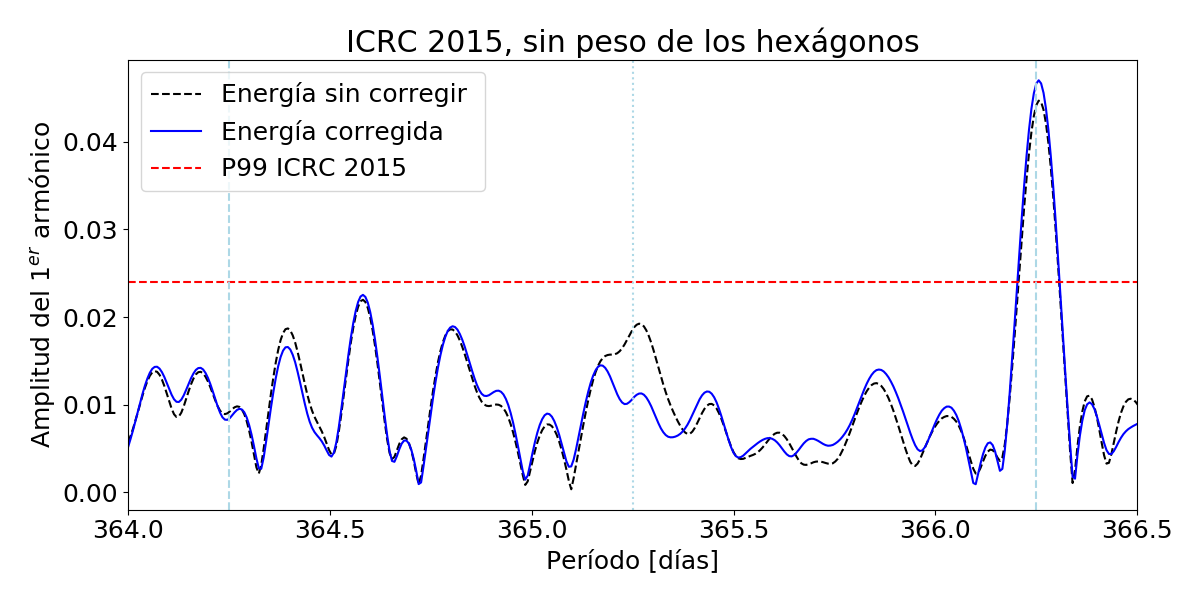
\includegraphics[width=0.6\textwidth]{../Anisotropia/ICRC/ICRC2017_Ecor_Eraw.png}
						\caption{Sin peso de la cantidad de tanques activos. } 	\label{fig:8EeV_sin_peso_ICRC2017_raw}
					\end{subfigure}%
				
					\begin{subfigure}[b]{\textwidth}
					\centering
						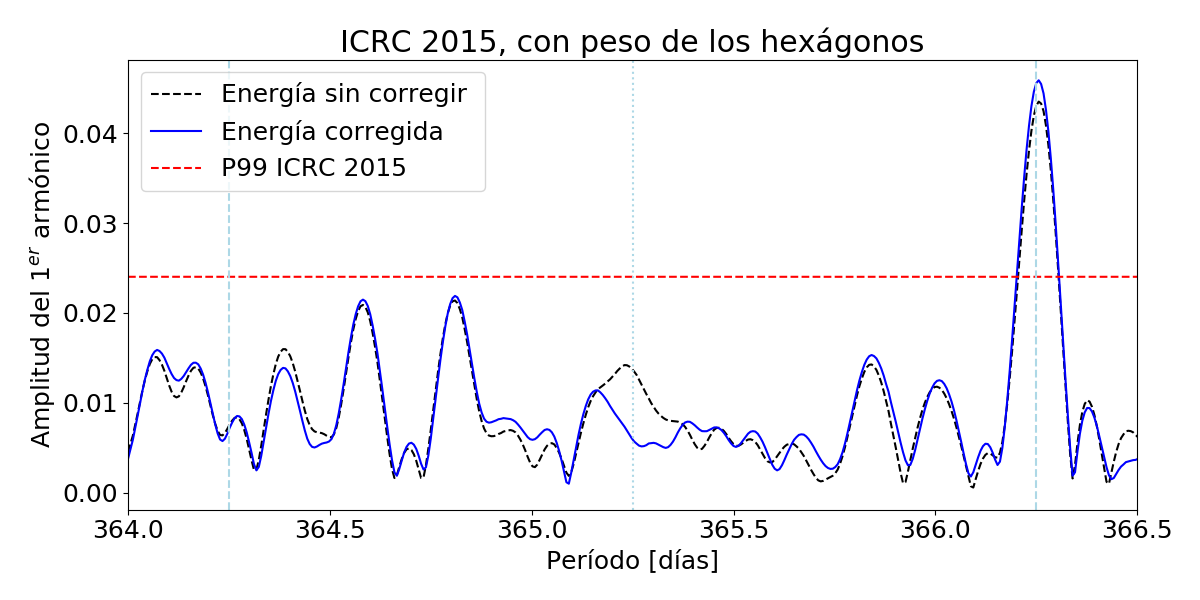
\includegraphics[width=0.6\textwidth]{../Anisotropia/ICRC/ICRC2017_Ecor_Eraw_hex.png}
						\caption{Con peso de la cantidad de tanques activos. } 	\label{fig:8EeV_sin_peso_ICRC2017_cor}
					\end{subfigure}
					\caption{Primer armónico en ascensión recta de los datos del ICRC 2017}
				\end{figure}

			Con esto podemos decir que el código para la anisotropía funciona para el caso donde no se considera los hexágonos. No tengo un referencia para comparar las anisotropías con el peso de los hexágonos, solamente el valor del pico del dipolo.

% ------> ICRC 2019
			\subsubsection{Resultados para los datos del ICRC 2019}
			
			Este es el conjunto de archivos donde se hicieron modificaciones como el uso de una nueva reconstrucción y la corrección del clima. Usé solamente los eventos 6T5. El rango de tiempo en el cual hice  el análisis es entre 1072969615 y 1535789456 (	2004-01-01 15:06:55 y 	2018-09-01 08:10:56)

			\begin{figure}[H]
				\centering
				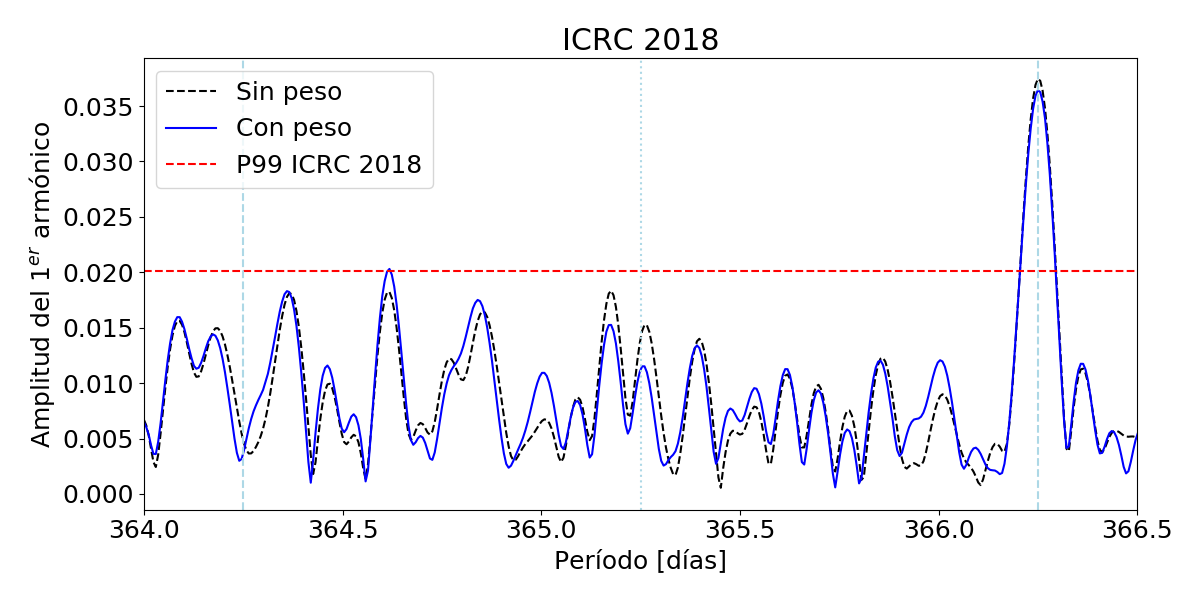
\includegraphics[width=0.6\textwidth]{../Anisotropia/ICRC/ICRC2019_Eraw_Eraw_hex.png}
				\caption{Primer armónico en ascensión recta de los datos del ICRC 2019.} \label{fig:8EeV_con_peso_ICRC2019}
			\end{figure}


			
% RESULTADOS PARA ANISOTROPÍAS EN RA PARA ALL TRIGGERS
	\section{Anisotropías en ascensión recta en los archivos con todos los disparos}
% ---> CARACTERISTICAS
		\subsection{Características de los archivos de datos analizados}

			Tenemos que tener en cuenta el archivo de datos de todos los disparos es entre los años 2013 y 2019, por lo que no podemos comparar los análisis de anisotropía con el conjunto  de datos del ICRC 2019 completo. Por lo que para compararlos, voy a hacer el análisis de ambos conjuntos de datos en el mismo rango de tiempo. Voy a hacer esto para poder comparar lo que sale. 			Este rango donde se está comparando entre archivo empieza en  $utc_i = 1372699409 $.

		%CARACTERISTICAS GENERALES DE AMBOS SET DE DATOS.

			A continuación se presentan las características de los archivos estudiados, sin ningún filtro de energía, sin acotar por tiempo. 

			\begin{table}[H]
			\centering
				\begin{tabular}{c|c|c|c}
				\textbf{Archivo} & \text{Eventos} & UTC inicial &  UTC final  \\ \hline
				2020			 & 13 739 351	  &  1372680068	&  1577879983 \\
				2019			 & 	8 463 063	  &	 1372680068 &  1496318388 \\
				2017			 &	8 592 302	  &  1372680068 &  1498521517 \\
					\end{tabular}
			\end{table}
			
			Puede verse que el Archivo de 2020 tiene más eventos, y además de tener un rango de tiempo mayor que el archivo del 2017 y 2019. Los archivos 2017 y 2019  tienen $7\,072\,964$ eventos coincidentes y los archivos 2017 y 2020 tienen $6\,902\,21$ A continuación se compara la diferencia de energía y la calibración entre estos eventos.

		%COMPARANDO DELTA E ENTRE LOS DOS ARCHIVOS
			En las  Figs.\,\ref{fig:deltaE} y \ref{fig:histograma} se muestra la diferencia entre el valor de energía entre eventos coincidentes entre los archivos 2017 y 2020. Puede apreciarse que la diferencia no esta centrada 0 y no aparenta tener una modulación del clima. Por lo tanto la diferencia se debe a una reconstrucción distinta de los eventos.

					\begin{figure}[H]
						\begin{subfigure}[b]{0.5\textwidth}
							\centering
							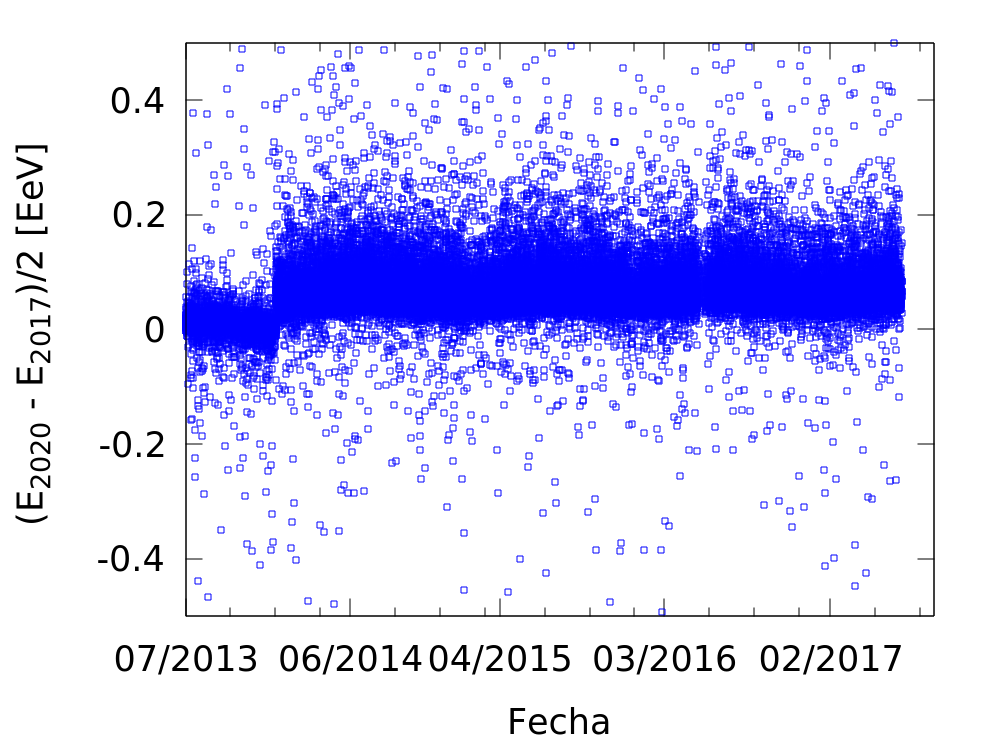
\includegraphics[width=\textwidth]{../Anisotropia/comparacion_deltaE.png}
							\caption{Diferencia entre las energías} \label{fig:deltaE}
						\end{subfigure}%
						\begin{subfigure}[b]{0.5\textwidth}
							\centering
							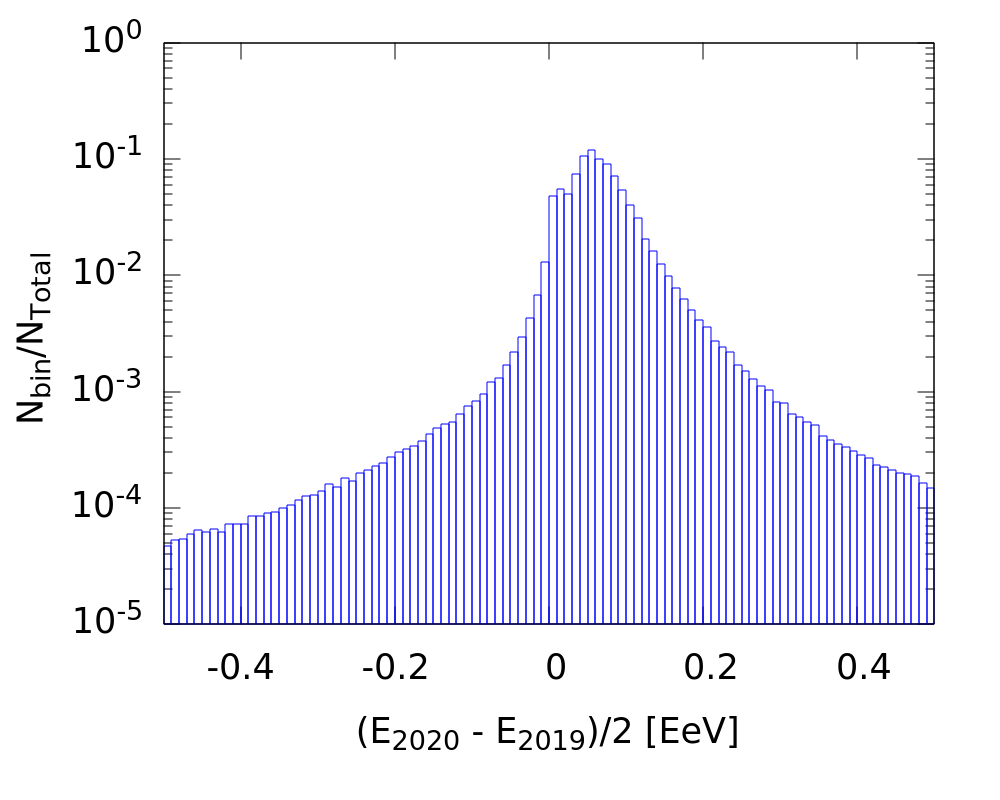
\includegraphics[width=0.8\textwidth]{../Anisotropia/histograma_deltaE.png}
							\caption{Histograma de las diferencias} 	\label{fig:histograma}
						\end{subfigure}
						\caption{Diferencia entre las energías del archivo de 2017 y el archivo del 2019}
					\end{figure}

		%COMPARANDO LA CURVA DE CALIBRACIÓN ENTRE LOS DOS ARCHIVOS
			Puede verse en la Fig.\,\ref{fig:calibracionE} que la curva de calibración entre ambos archivos es distinta, ya que la coordenada al origen como la pendiente es difieren entre para ambos archivos. Esto implica que los valores A y B de la curva $E=A\times (S_{38})^B$ son distintos para ambos conjunto de datos, ¿en qué afectaría? en primer lugar en el valor de la energía, segundo en análisis que dependan del estos parámetros como el análisis de la modulación del clima.

				\begin{figure}[H]
					\centering
					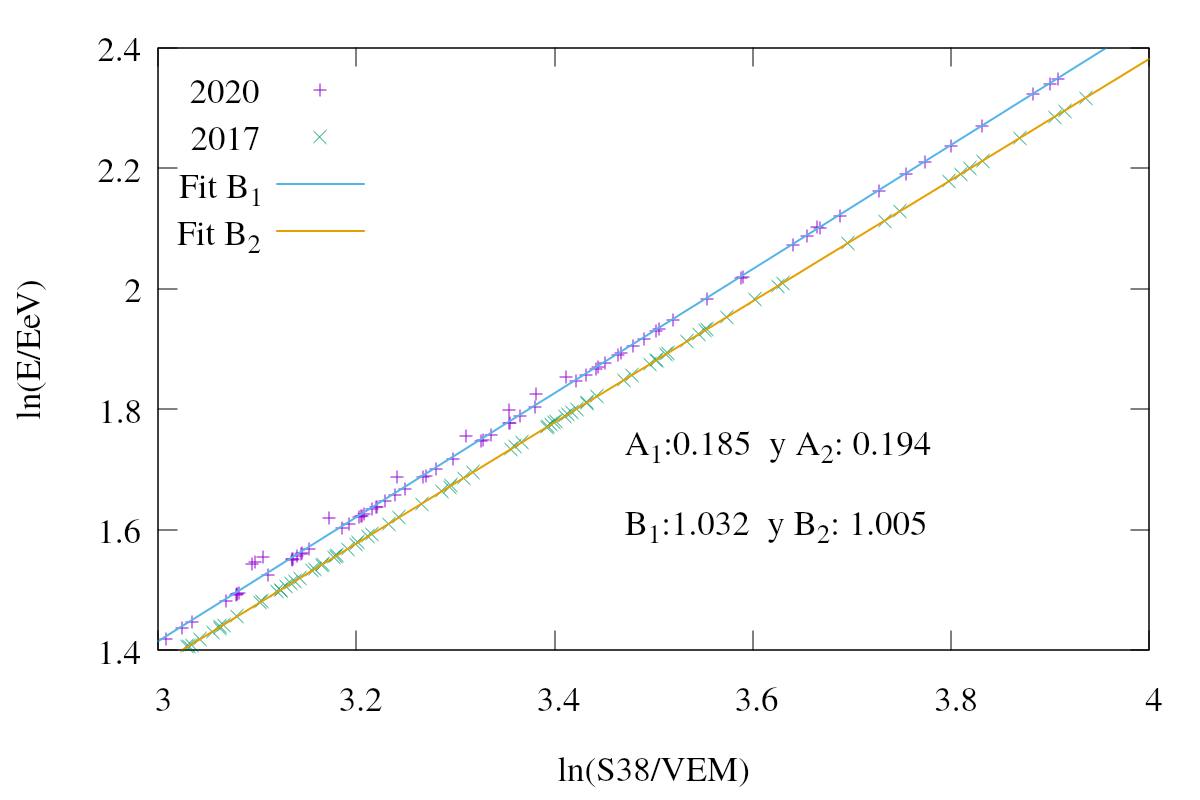
\includegraphics[width=0.65\textwidth]{../Anisotropia/comparacion_reconstruccion.png}
					\caption{Calibración de las energías del archivo de 2017 y el archivo del 2019}
					\label{fig:calibracionE}
				\end{figure}

% ---> 1 EeV 
		\subsection{Eventos por encima de 1 EeV }
% ------> CARACTERISTICAS
			\subsubsection{Características de los datos analizados}

			Comparando las cantidad de eventos por encima de 1 EeV para cada conjunto de datos

				\begin{table}[H]
					\centering
						\begin{tabular}{c|c|c|c}
						\textbf{Archivo} & \text{Eventos} 	& UTC inicial &  UTC final  \\ \hline
						2020			 & 1\,515\,872		& 1372680308  & 1577879886 \\
						%2019			 & 647\, 656		& 1372699410  & 1496267276 \\
						2017			 & 635\, 353		& 1372680308  & 1496275090 \\
						\end{tabular}
				\end{table}

{\bf hasta acá está verificado}
% ------> ALL TRIGGERS 2017
			\subsubsection{Resultados del archivo de 2017}

				\begin{figure}[H]
					\centering
					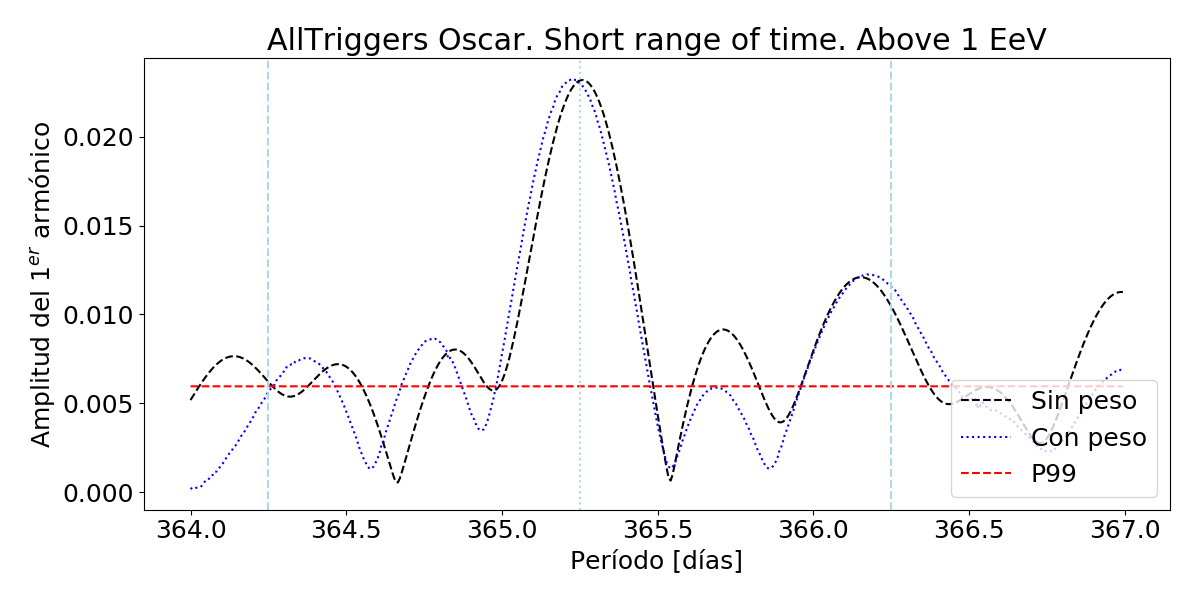
\includegraphics[width=0.6\textwidth]{../Anisotropia/AllTriggers/AllTriggers_2017_Short_range_Above_1_EeV.png}
				\end{figure}
			En el gráfico de todos los disparos para el archivo de 2017, se ve que hay una modulación anual importante. Es de esperarse ya que la correción del clima aun no fue implementada para este conjuntos de datos.

			Comentario: {\sl Para el análisis en frecuencias, no hace ruido el hecho que la línea del P99 esté tan bajo, siendo que solo depende de la cantidad de eventos, }


% ------> ALL TRIGGERS 2019
		%\subsubsection{Resultados del archivo del 2020}

		%{\bf Esta sección no fue actualizada aún}
		%	\begin{figure}[H]
		%		\centering
		%		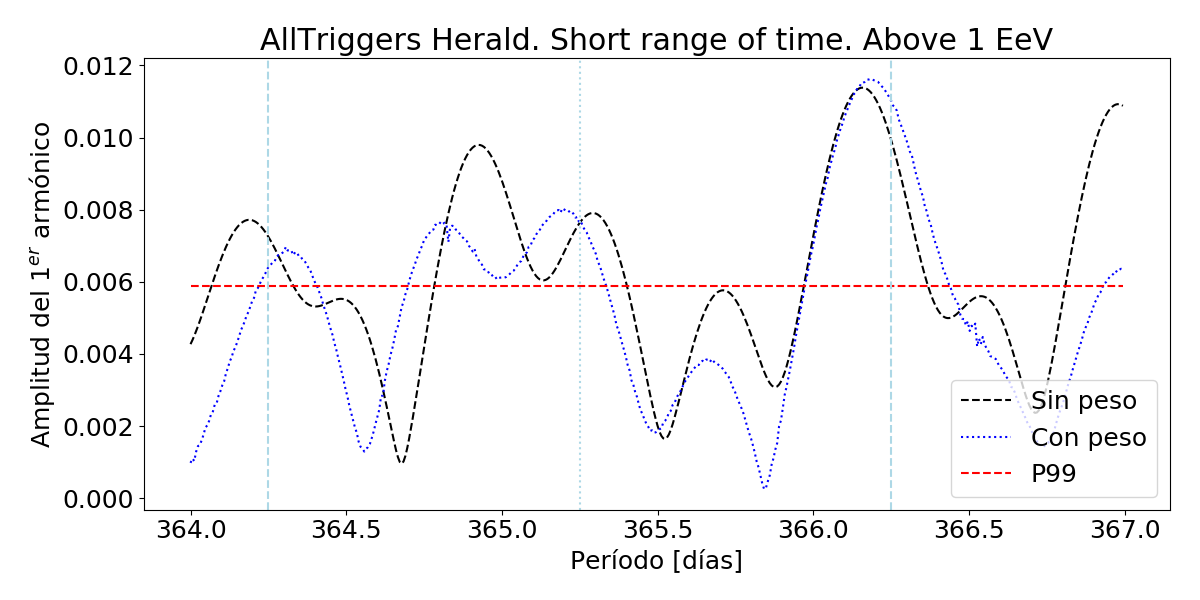
\includegraphics[width=0.95\textwidth]{../Anisotropia/AllTriggers/AllTriggers_2019_Short_range_Above_1_EeV.png}
		%	\end{figure}

% --> WEATHER STUFF

			\subsubsection{Modulación del clima para todos los triggers}




			Para corroborar los parámetros del clima, primero calculé las tasas de eventos de los archivos del 2017 y 2020 para energías mayores a 1  EeV, donde obtuve los siguientes gráficos Fig.\ref{fig:rate_daily_2017_1EeV} y \ref{fig:rate_daily_2020_1EeV}. 

				\begin{figure}[H]
				
					\begin{subfigure}[b]{0.5\textwidth}
					\centering
					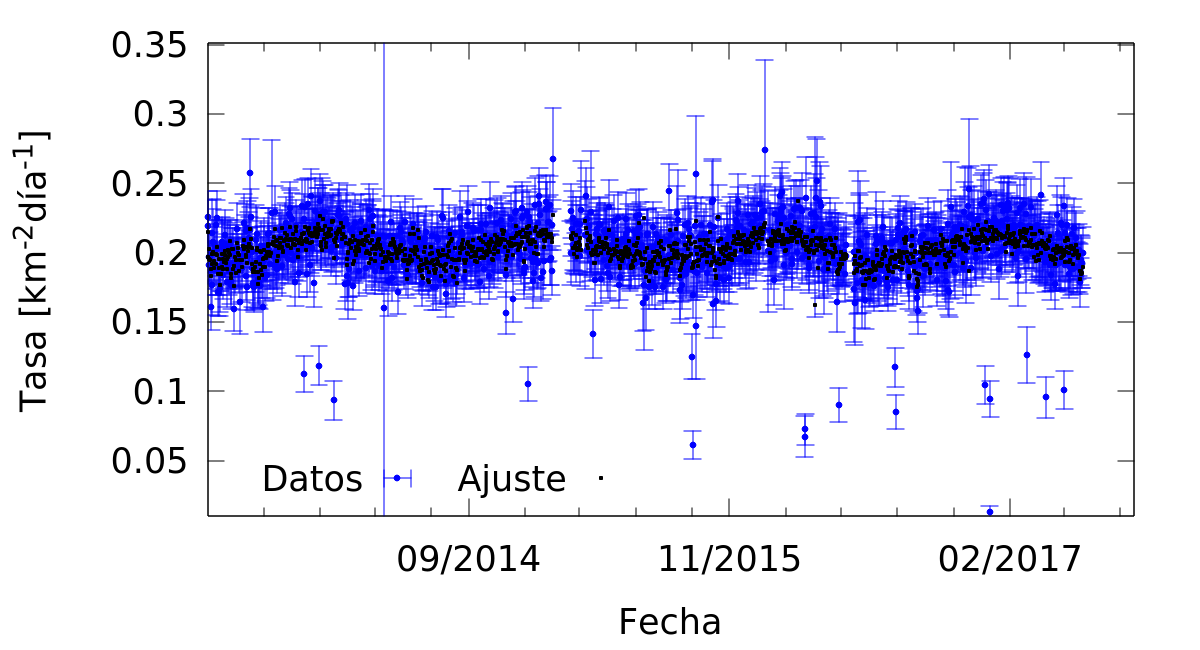
\includegraphics[width=\textwidth]{../Anisotropia/daily_rate/daily_rate_AllTriggers_2017_1EeV.png}
					\caption{Archivo de 2017} 	\label{fig:rate_daily_2017_1EeV}
					\end{subfigure}%
				\hfill
					\begin{subfigure}[b]{0.5\textwidth}
					\centering
					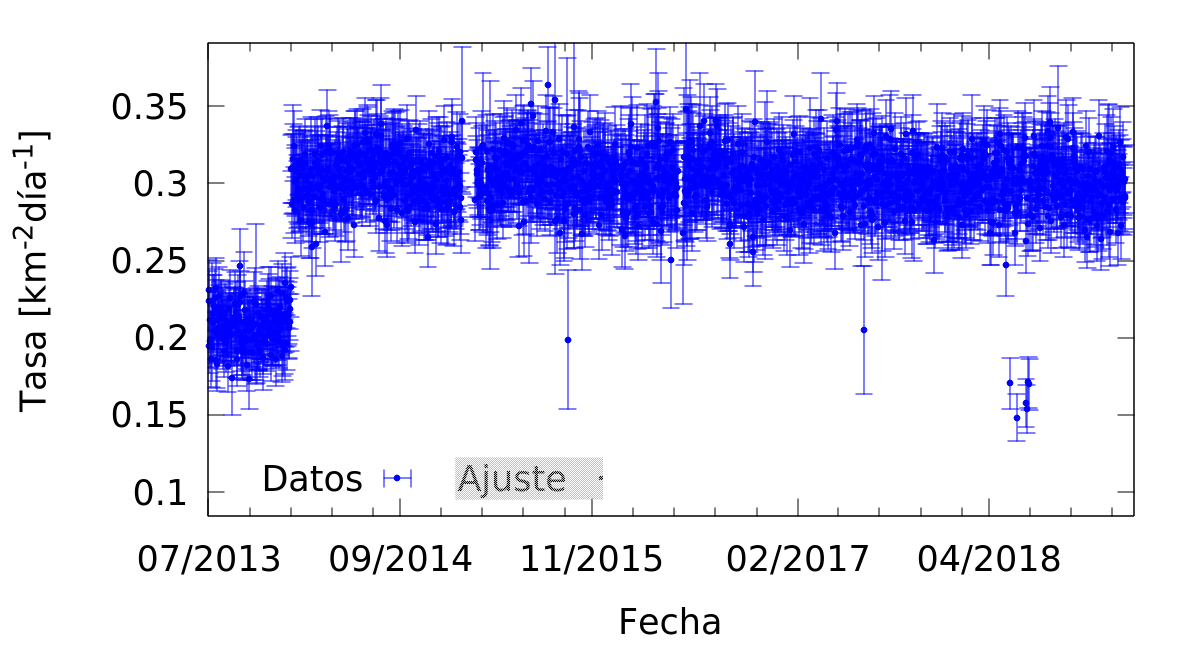
\includegraphics[width=\textwidth]{../Anisotropia/daily_rate/daily_rate_AllTriggers_2019_1EeV.png}
					\caption{Archivo del 2020} 	\label{fig:rate_daily_2020_1EeV}
					\end{subfigure}
					\caption{Tasa de eventos diaria por encima de 1 EeV para los datos de todos los disparos.}
				\end{figure}

			Después calculé los parámetros del clima para energía mayores a 1 EeV. Para el archivo de 2017 obtuve la Fig.\,\ref{fig:parameters_2017_1EeV}. Los comparé con el paper del weather del main array, para ver si dan algo razonable. Verifiqué las siguientes cosas para el ajuste

			\begin{itemize}
				\item Me fijé que delay en la densidad cada momento fuera de dos  horas
				\item Me fijé que el ajuste no tuviera en cuenta periodos malos, bad periods
				\item Me fijé que el delay de la densidad media también fuera tal que para cada evento estuviera centrada $\pm$12 horas
				\item También me fijé que el rango de tiempo estuviera bien, porque estos datos están disponibles desde el 2013  recién
				\item Me fijé que los $\chi^2$ reducido fuera algo razonable. Todos rondaban alrededor de $1.05$
			\end{itemize}

			EL rango de tiempo que usé fue este: 
			\begin{itemize}
				\item Inicio: 1372680308
				\item Final: 1496275090
			\end{itemize}
				\begin{figure}[H]
					\begin{subfigure}[b]{0.5\textwidth}
					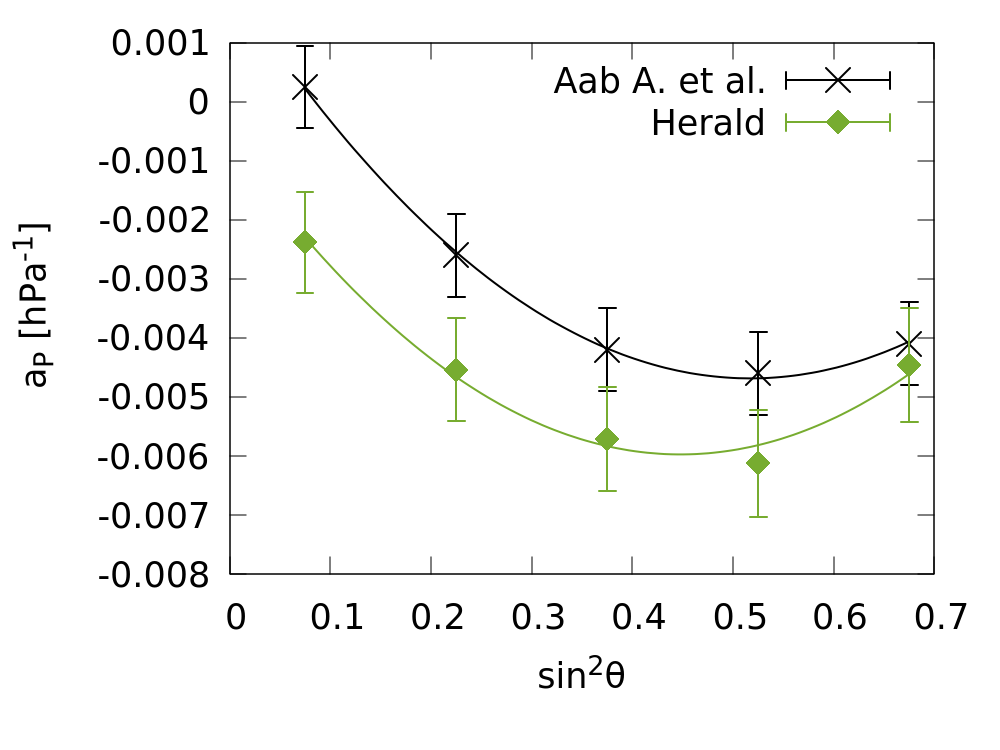
\includegraphics[width=\linewidth]{../Anisotropia/params/ap_2017_above_1EeV.png}
					\caption{Parámetro $a_P$ }
					\label{fig:ap_2017_1EeV}
					\end{subfigure}%
					\hspace{\fill}
					\begin{subfigure}[b]{0.5\textwidth}
					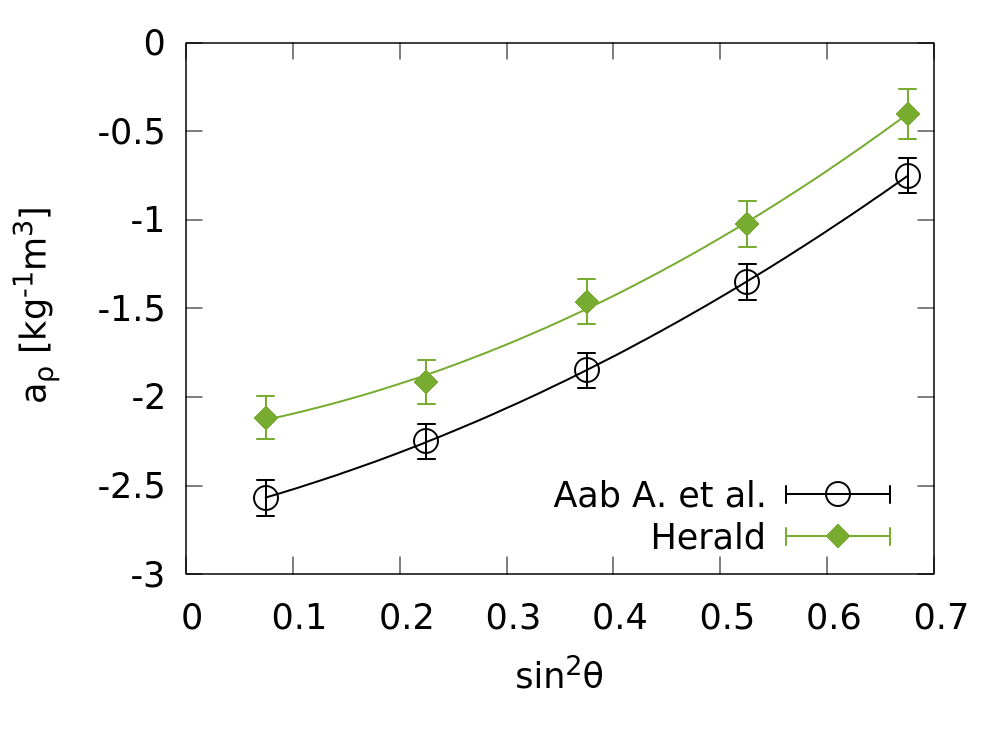
\includegraphics[width=\linewidth]{../Anisotropia/params/arho_2017_above_1EeV.png}
					\caption{Parámetro $a_{\rho}$ }
					\label{fig:arho_2017_1EeV}
					\end{subfigure}%
					\hspace{\fill}
					\begin{subfigure}[b]{\textwidth}
					\centering
					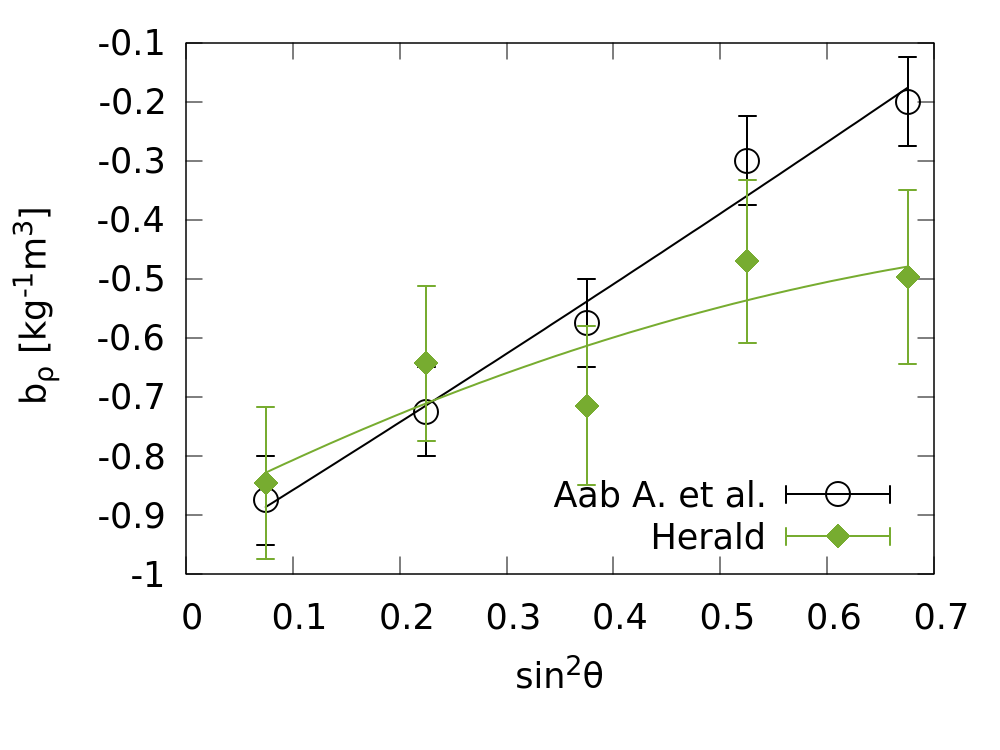
\includegraphics[width=0.5\linewidth]{../Anisotropia/params/brho_2017_above_1EeV.png}
					\caption{Parámetro  $b_\rho$	 }
					\label{fig:brho_2017_1EeV}
					\end{subfigure}%
					\caption{Parámetros de la modulación del clima considerando los datos para todos los disparos de 2017. Los mismos se comparan con los ajustes obtenidos en \cite{aab2017impact}.}\label{fig:parameters_2017_1EeV}
				\end{figure}

				Lo que más me llama la atención es el comportamiento del parámetro $b_\rho$, que como se discutió en otras oportunidades, tiene que ver con el parámetro $a_\rho$ con una razón de  $1:3$ más o menos. 



			Hacemos el mismo procedimiento con el archivo 2020, {\bf pero filtrando los eventos por el valor de S38 sin corregir por la modulación del clima}. Para calcular la tasa y los parámetros del clima, se toman los eventos después de ese salto de 0.2 a 0.3, obtengo los siguientes resultados:

				\begin{figure}[H]
					\centering
					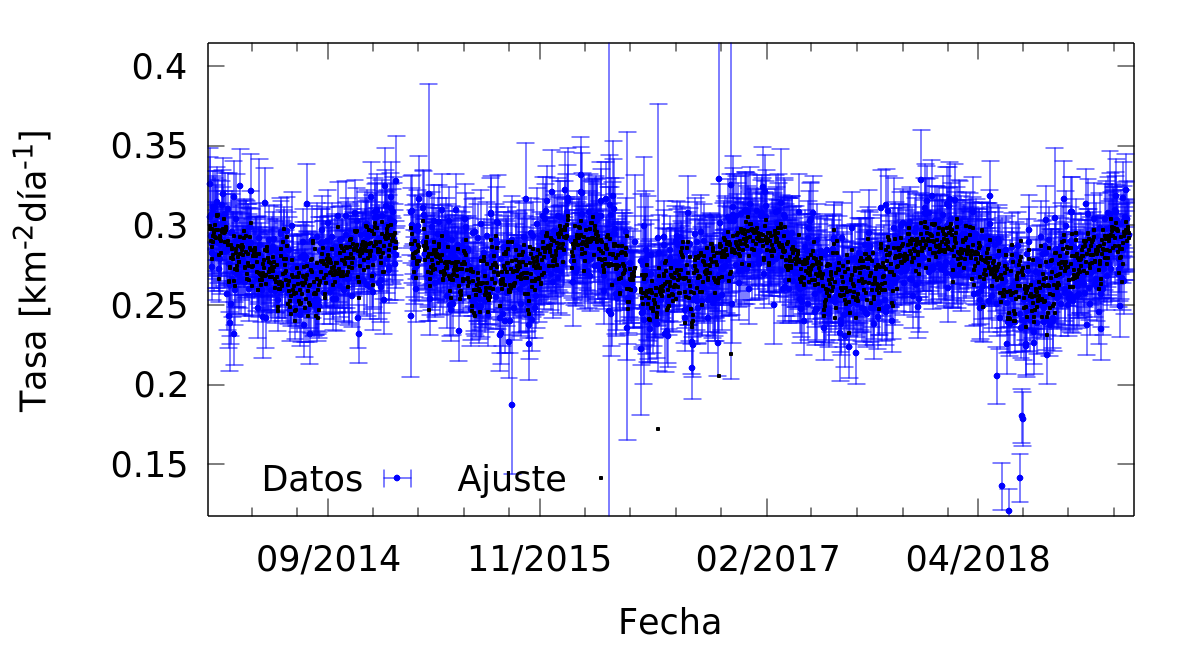
\includegraphics[width=0.5\textwidth]{../Anisotropia/daily_rate/daily_rate_AllTriggers_2020_1EeV.png}
				\end{figure}

			Acá también verifiqué lo mismo que el caso anterior, lo único que ahora el $\chi^2$ rondaba alrededor de los $1.08$. Siempre verifico que no sea mucho mayor o menor a 1.

			EL rango de tiempo que usé para este caso fue este: 
			\begin{itemize}
				\item Inicio: 1388910508
				\item Final: 1550490858
			\end{itemize}
			
				\begin{figure}[H]
					\begin{subfigure}[b]{0.5\textwidth}
					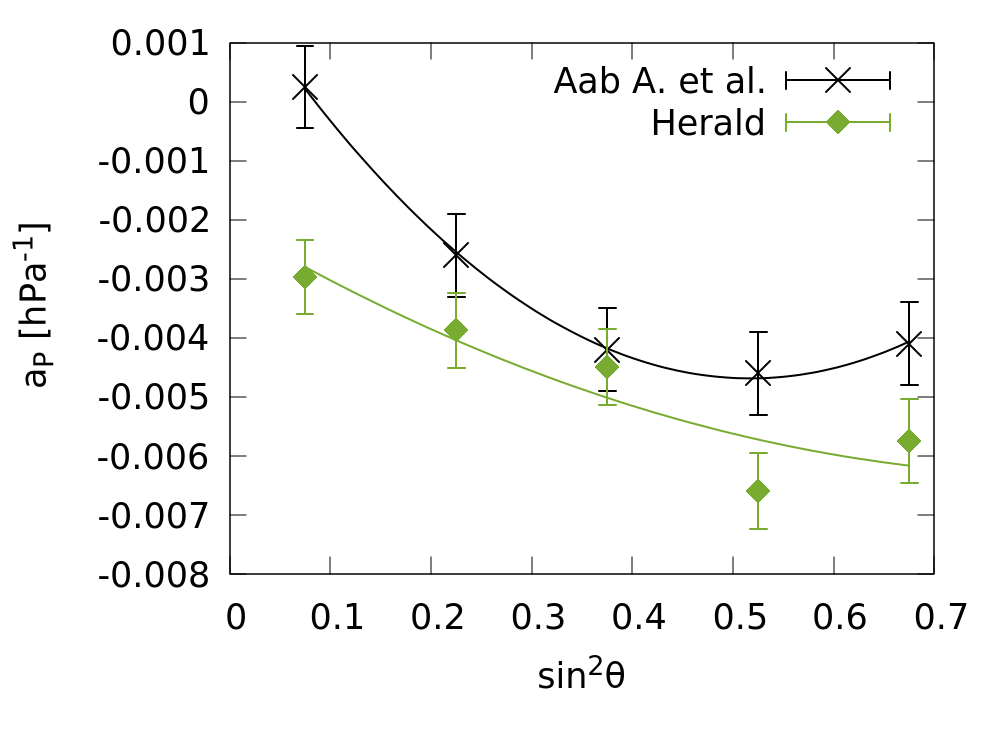
\includegraphics[width=\linewidth]{../Anisotropia/params/ap_2020_above_1EeV.png}
					\caption{Parámetro $a_P$ }
					\label{fig:ap_2020_1EeV}
					\end{subfigure}%
					\hspace{\fill}
					\begin{subfigure}[b]{0.5\textwidth}
					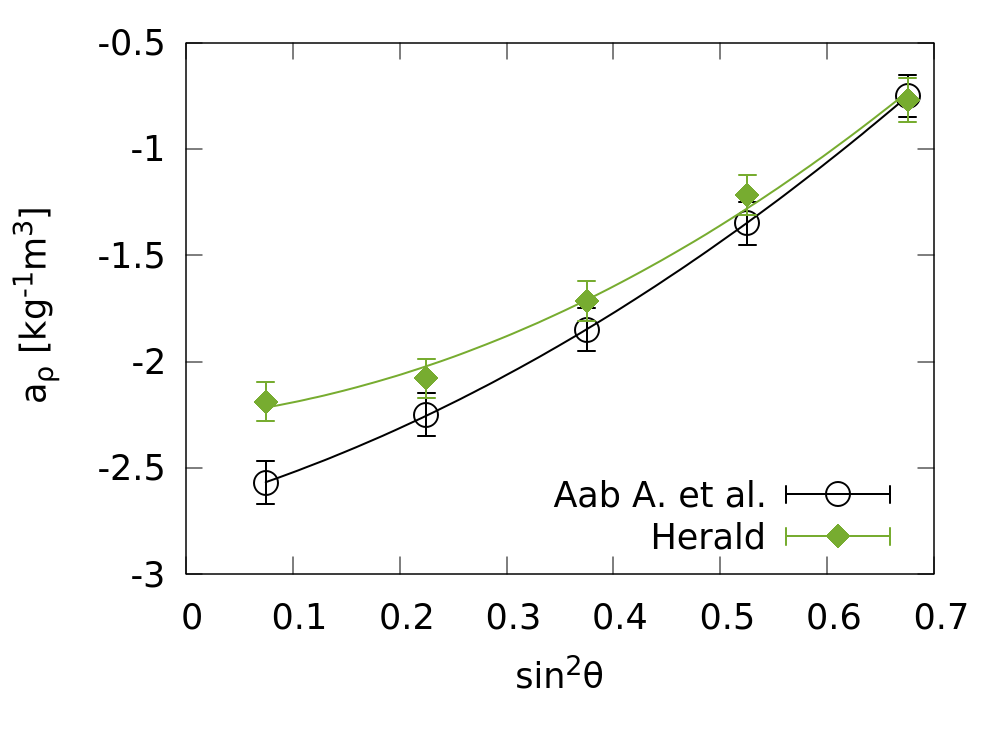
\includegraphics[width=\linewidth]{../Anisotropia/params/arho_2020_above_1EeV.png}
					\caption{Parámetro $a_{\rho}$ }
					\label{fig:arho_2020_1EeV}
					\end{subfigure}%
					\hspace{\fill}
					\begin{subfigure}[b]{\textwidth}
					\centering
					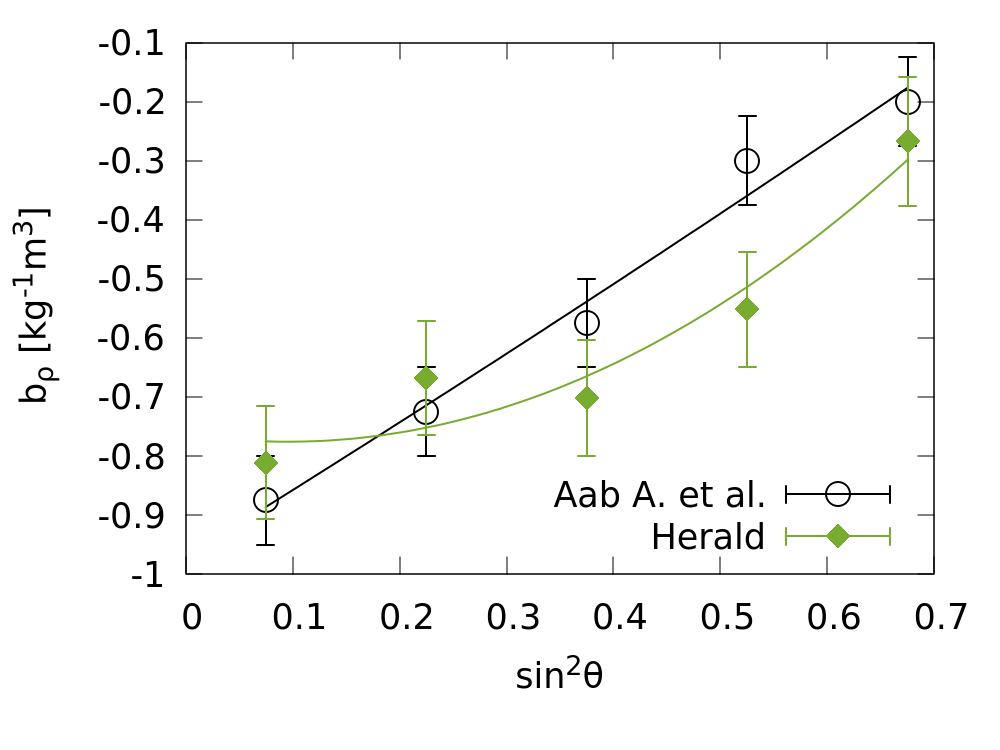
\includegraphics[width=0.5\linewidth]{../Anisotropia/params/brho_2020_above_1EeV.png}
					\caption{Parámetro  $b_\rho$	 }
					\label{fig:brho_2020_1EeV}
					\end{subfigure}%
					\caption{Parámetros de la modulación del clima considerando los datos para todos los disparos de 2020. Los mismos se comparan con los ajustes obtenidos en \cite{aab2017impact}.}\label{fig:parameters_2020_1EeV}
				\end{figure}



			Considerando el filtro con el S38 en el archivo 2020 y la energía en el 2017, quiero saber si obtengo parametros  del clima comparables. Ya que el Main Array se corresponden los parametros del 2015 y 2019, yo esperaría que con todos los triggers pase los mismo. Una diferencia importante entre ambos análisis es que los parametros del 2020 contienen eventos hasta el 31/12/2019.


				\begin{figure}[H]
					\begin{subfigure}[b]{0.5\textwidth}
					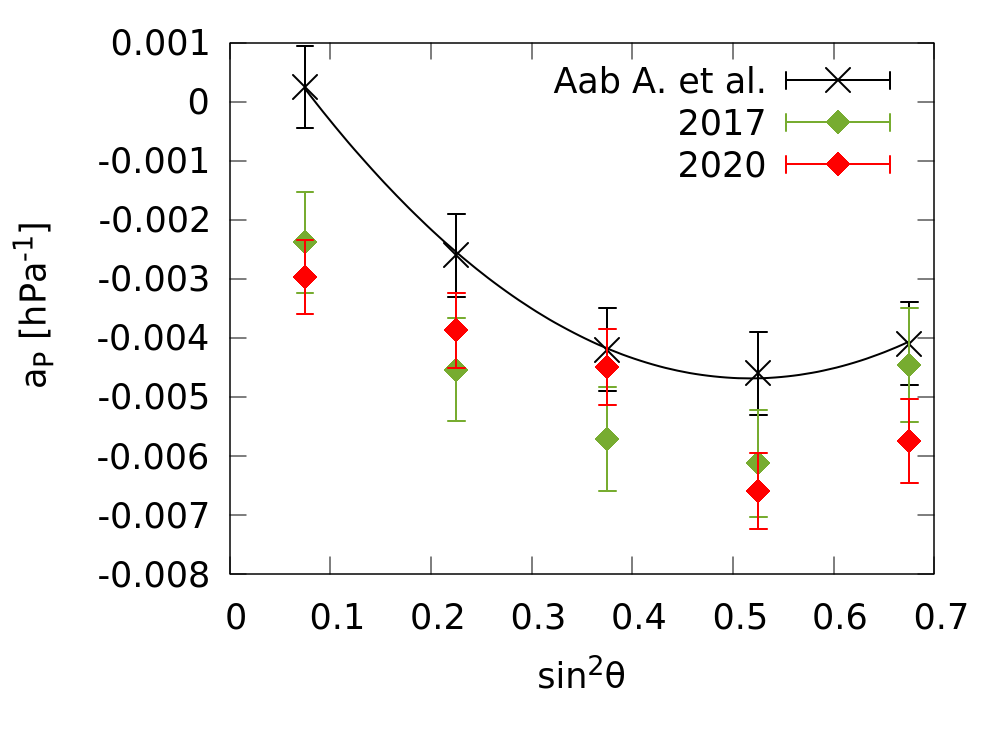
\includegraphics[width=\linewidth]{../Anisotropia/params/ap_2017_2020_above_1EeV.png}
					\caption{Parámetro $a_P$ }
					\end{subfigure}%
					\hspace{\fill}
					\begin{subfigure}[b]{0.5\textwidth}
					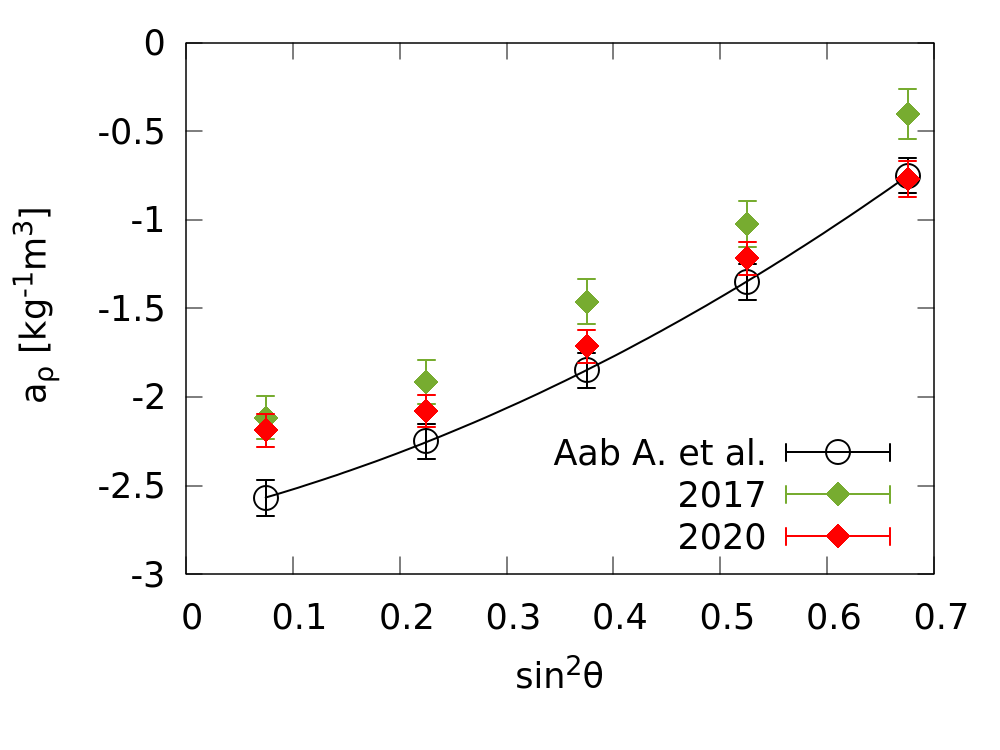
\includegraphics[width=\linewidth]{../Anisotropia/params/arho_2017_2020_above_1EeV.png}
					\caption{Parámetro $a_{\rho}$ }
					\end{subfigure}%
					\hspace{\fill}
					\begin{subfigure}[b]{\textwidth}
					\centering
					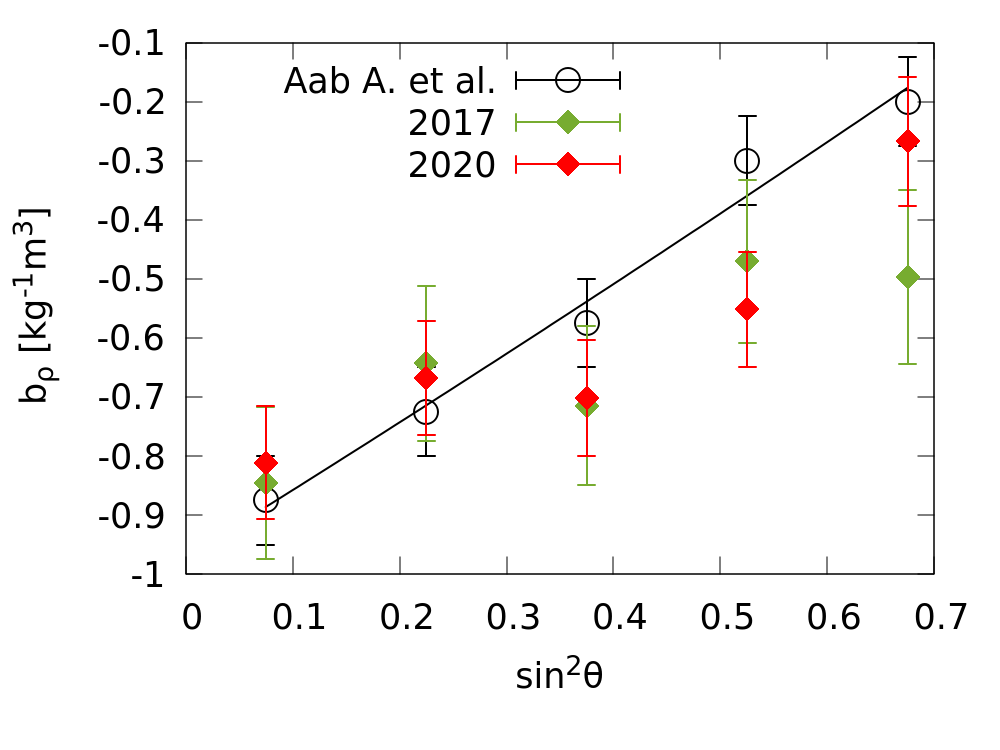
\includegraphics[width=0.5\linewidth]{../Anisotropia/params/brho_2017_2020_above_1EeV.png}
					\caption{Parámetro  $b_\rho$	 }
					\end{subfigure}%
					\caption{Parámetros de la modulación del clima considerando los datos para todos los disparos del archivo 2017 y 2020. Los mismos se comparan con los ajustes obtenidos en \cite{aab2017impact}.}
				\end{figure}

			Se ve que estos parametros no son comparables. 

{\bf Hasta acá está verificado}


\subsubsection*{To do list }
		\begin{itemize}
			\done (DONE) ¿estoy haciendo bien la cuenta? 
			\done (DONE) el log en ln o log10 para cpp? es ln==log en cpp
			\done¿Hay algo en la aproximación de rayleigh que se pasó por alto? Sigo buscando
			\done (DONE?) ¿Entiendo bien la approx? --Creo que sí, leí el paper que referencian, pero puede que un detalle se me halla escapado
	\item Hacer 4-8 EeV
	\done Comparar con ICRC por debajo de full efficency (¿necesario?): {\sl No, no es necesario}
	\done Entender que está pasando con el percentil 99 : {\sl Se discutió con Mollerach}
	\done {\sl (DONE)} Actualizar los gráficos para long range 
	\done {\sl (DONE sort of)} Verificar el weather de AllTriggers2017 por encima de 1 EeV
	\item Empezar el código para analizar más momentos (dipole, quadruplo): {\sl work in progress}
	\done {\sl (DONE)} Mandar mail
	\done Actualizar los rango de tiempo del ICRC 2019 y el AllTriggers 2019
\end{itemize}



\subsubsection*{How to do the analisis right?}

\begin{itemize}
	\done Fijate que el rango de tiempo esté bien
	\done Asegurate que los archivos esten actualizados a la fecha que queres analizar.
	\done Fijarse si tengo que usar 5t5 o 6t5
\end{itemize}

\subsubsection*{Comentarios importantes}

\begin{itemize}
	\item Para el rango de energía 2 EeV para arriba usamos el  Main\_Array, porque ya es más o menos full eficiency
	\item En el bin de energía entre 1\,EeV y 2\,EeV usamos el archivo AllTriggers
	\item Tengo ambos archivos hasta el 31 12 2019, así también como el archivo del clima actualizado hasta  Monday, 18 February 2019 23:55:00
\end{itemize}



{\bf 1395680272} CHECK THIS EVENT!!!!!!!!!!!